%!TEX root = ../template.tex
%%%%%%%%%%%%%%%%%%%%%%%%%%%%%%%%%%%%%%%%%%%%%%%%%%%%%%%%%%%%%%%%%%%%
%% 3-Background_Work.tex
%% NOVA thesis document file
%%
%% Chapter with the background work that is not necessary state of the art stuff but necessary for the explanation of the work done chapter.
%%%%%%%%%%%%%%%%%%%%%%%%%%%%%%%%%%%%%%%%%%%%%%%%%%%%%%%%%%%%%%%%%%%%

\typeout{NT FILE 3-Background.tex}%

\chapter{Background}
\label{cha:Background}

\glsresetall

\section{Introduction}
\label{sec.3:Introduction}

Several concepts are required for a proper understanding of this thesis, some of which have not yet been introduced in the state of the art presented in Chapter~\ref{cha:State of the art}. These include methods for spacing agents on the two-sphere (Section~\ref{sec.3:Direct computation agent spacing on the two-sphere} and Section~\ref{sec.3:Iterative computation agent spacing on the two-sphere}), the drone model considered in this work (Section~\ref{sec.3:Vehicle model and noninear control}), the vehicle model and nonlinear controller architecture (Section~\ref{sec.3:Vehicle model and noninear control}), Lyapunov stability theory (Section~\ref{sec.3:Lyapunov Stability and Lyapunov-Based Control}), network topologies \ref{sec.3:Network topologies} and consensus-based coordination algorithms (Section~\ref{sec.3:Consensus-Based Coordination}).

Before these techniques are introduced in detail, a brief contextualization is provided to clarify their role within the overall control architecture.The approach followed in this thesis relies on three main components that are not extensively covered in the state of the art. 

The first issue concerns the positioning of agents on the surface of a mesh (typically a sphere). This positioning defines the final desired configuration of the agents during target encirclement and therefore requires methods capable of generating points with near-uniform separation on the spherical surface. As previously mentioned in the introduction \ref{cha:introduction}, the adoption of a near-uniform distribution is motivated by the uncertainty associated with the target dynamics, since only the target position is assumed to be known. Because the maneuvering capabilities and future motion of the target are unknown, an approximately uniform distribution of agents around the target provides balanced spatial coverage and reduces directional bias in the encirclement configuration. Consequently, regardless of the target's motion direction, the collective reachability set of the agents remains approximately evenly distributed around the target, improving the robustness of the encirclement strategy.

The second component is the dynamical model of the drones (Section~\ref{sec.3:Vehicle model and noninear control}), which is shared by both the target and the pursuing agents. This model underlies the design of the control laws and ensures consistency across all simulated agents, as well as the internal drone controller, introduced in Section~\ref{sec.3:Vehicle model and noninear control}, responsible for converting a desired position reference into appropriate actuator commands that drive the quadrotor to the target position. Since this inner-loop controller naturally induces straight-line motion toward the reference, an additional control layer is required to shape the resulting trajectories.

Finally the in between trajectory controller, mentioned in Section~\ref{sec.3:Lyapunov Stability and Lyapunov-Based Control}, provides reference positions to the quadrotor and ensures convergence to a desired location \gls{p_desired}, this controller exists only for the centralized and decentralized versions of the architecture not the generalized non sphere specific one. This controller however, does not guarantee collision-free motion. For example, intersecting paths between agents and their respective goals may lead to collisions.

Other objective depended (centralized, decentralized, generalized) controllers exist for example the network topology and target estimation only apply to the decentralized and generalized while the mesh deformation and voronoi diagram only apply to the generalized.

In summary, the framework consists of three core elements: the computation of objective positions, the internal drone controller, and the intermediate trajectory controller that generates reference positions along the path from the current state to the desired point. Notably, a complete trajectory is never computed explicitly. Additional modules may be incorporated depending on the chosen architecture and objectives.

The sections that follow do not aim to provide a comprehensive treatment of the underlying theories. Instead, they introduce the essential concepts and tools required to fully understand the methods and results presented in Chapters \ref{cha:Centralized Development}, \ref{cha:Decentralized Development} and \ref{cha:Decentralized Development}.

\section{Direct computation agent spacing on the two-sphere} \label{sec.3:Direct computation agent spacing on the two-sphere}

In this section, several direct computation methods for distributing points on a manifold are discussed, this are methods that given a number of desired points will directly give the final distribution of the same. The primary objective is to achieve the most uniform spacing possible between agents. Such uniformity allows for more efficient use of each agent's reachability set at any given time. In other words, minimizing overlap between the reachability regions of different agents maximizes the collective coverage and effectiveness of the multi-agent system. For simplicity the two-sphere or unit sphere will be the main manifold considered since the problem at hand is encircling a target, where $\mathbb{S}^2 = \{\mathbf{x} \in \mathbb{R}^3 : \|\mathbf{x}\| = 1\}$ denotes the unit sphere (the 2-norm will be defined as $\|.\|$ from now on). Three different methods will be discusses, the latitude and longitude, the fibonacci sphere and poisson disk sampling.

\subsection{Latitude and Longitude} \label{sec.3:Latitude and longitude}

The latitude--longitude lattice method here mentioned, heavily inspired and influenced by \cite{Latitude_Longitude_vs_fibonacci}, consists of points located at the intersections of a grid of meridians and parallels, separated by equal angular increments in latitude and longitude. This arrangement might be referred as as the \emph{latitude--longitude grid} or the \emph{equal-angle grid}. Due to the convergence of meridians toward the poles, the density of points increases with latitude, resulting in significant anisotropy. 

The total number of points, denoted by $P$, depends on the angular spacing $\delta$ between adjacent grid lines. If the sphere is divided into $N$ equal angular intervals in latitude, so that $\delta = 180^\circ / k$ with $k = 1, 2, \ldots$, then the total number of grid points is

\begin{equation}
    P = 2N(N - 1) + 2, \quad N \in \mathbb{N}
\end{equation}

This expression accounts for the $2k$ meridians and the $k - 1$ parallels, along with the two poles. A limitation for the desired use case is that the total number of agents is constrained by the parameter $N$, which restricts the set of achievable formations. For example, configurations involving 3, 4, or 5 agents, cannot be realized within this framework $P \overset{N=1}{=} 2, P \overset{N=2}{=} 6$. As can be observed in Figure~\ref{fig.3:latlon_results_demonstration}, the spacing produced by this method is best demonstrated from a side view, where its clearly visible that the points are arranged in a grid-like pattern as well as their clumping around the edge of the circular projection.

\begin{figure}[htbp]
\centering
\subfloat[Normal]{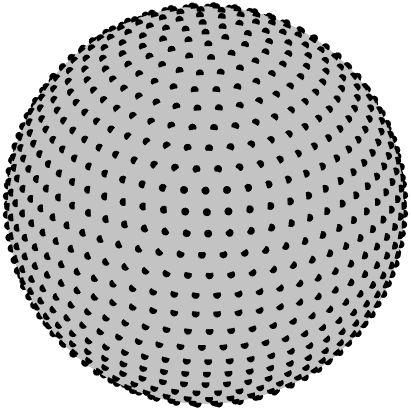
\includegraphics[width=3cm]{5-Figures/Chapter4/latlon_sphere/latlon_sphere_normal.png}}\hfil
\subfloat[Top]{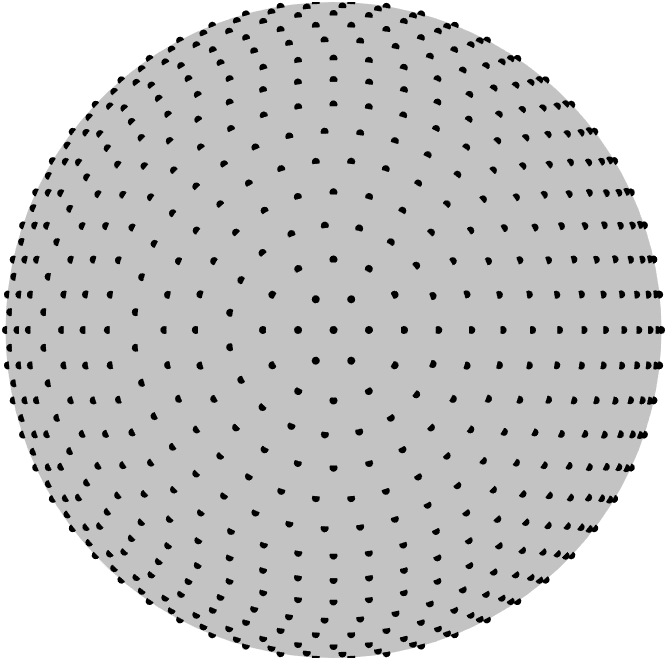
\includegraphics[width=3cm]{5-Figures/Chapter4/latlon_sphere/latlon_sphere_top.png}}\hfil 
\subfloat[Side]{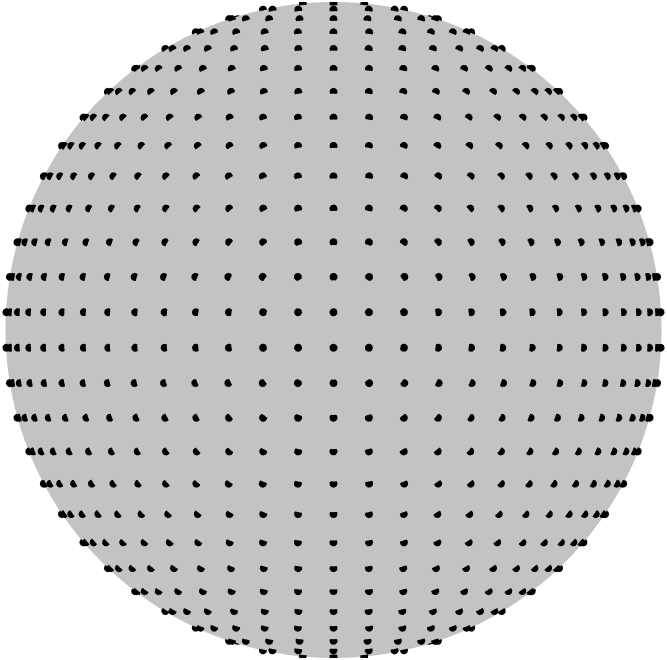
\includegraphics[width=3cm]{5-Figures/Chapter4/latlon_sphere/latlon_sphere_side.png}}
\caption{Latitude and Longitude demonstration (1070 points)}
\label{fig.3:latlon_results_demonstration}
\end{figure}

\subsection{Fibonacci Lattice}
\label{sec.3:Fibonacci Lattice}

The Fibonacci lattice, also heavily inspired and influenced by \cite{Latitude_Longitude_vs_fibonacci}, is named after the Fibonacci ratios, which was discovered in ancient India \cite{fibonacci_history}. The construction is based on the Fibonacci sequence, in which each term from the third onward is the sum of the two preceding terms:
\[
0, 1, 1, 2, 3, 5, 8, 13, 21, \ldots
\]

Given two consecutive Fibonacci numbers $F_i$ and $F_{i+1}$, the Fibonacci ratio is defined as $F_{i+1}/F_i$. As first proved by Robert Simson in 1753 \cite{fibonacci_to_golden_ratio_1,fibonacci_to_golden_ratio_2}, this ratio converges rapidly, as $i \to \infty$, to the golden ratio
\begin{equation}
  \varphi = 1 + \varphi^{-1} = \frac{1 + \sqrt{5}}{2} \simeq 1.618 .
  \label{eq:golden_ratio}
\end{equation}

The Fibonacci lattice differs in the use of the \emph{golden angle} along the spiral lattice on the sphere where the longitudinal rotation between consecutive points along the generating spiral is given by \eqref{eq.3:golden_angle}, 
or, equivalently, its complementary angle.

\begin{equation}
  360^\circ \left(1 - \varphi^{-1}\right)
  = 360^\circ \varphi^{-2}
  \simeq 137.5^\circ ,
  \label{eq.3:golden_angle}
\end{equation}

\begin{equation*}
  360^\circ \varphi^{-1} \simeq 222.5^\circ .
  \label{eq.3:golden_angle_complementary}
\end{equation*}

In some lattice constructions, the golden ratio $\varphi$ is replaced by a rational approximant given by a Fibonacci ratio; this is the case when the total number of points is constrained to be a Fibonacci number. But why use the golden angle as the spacing between points in the sphere lattice? Since the golden angle optimizes packing efficiency in spiral lattices, due to being the golden ratio the \emph{most irrational} number, the  periodic or near-periodic alignments in the spiral structure is avoided. As a result, lattice points do not cluster, and spatial uniformity is preserved.

When a Fibonacci ratio is employed, the total number of lattice points is $F + 1$, where $F > 1$ is a Fibonacci number. In contrast, the lattice used in this work is based directly on the golden ratio and admits any odd number of points.

To construct the lattice, let $N$ be a natural number and let the integer index $i$ range from $-N$ to $+N$. 

The spherical coordinates (in radians) of the $i$th point are given by Equation~\eqref{eq.3:fibonacci_lat_lon} being the total number of points defined by \eqref{eq.3:fibonacci_number_of_points}.

\begin{align}
    \text{lat}_i &= \arcsin\!\left(\frac{2i}{2N + 1}\right), \\
    \text{lon}_i &= 2\pi i \varphi^{-1} .
    \label{eq.3:fibonacci_lat_lon}
\end{align}

\begin{equation}
    P = 2N + 1 
    \label{eq.3:fibonacci_number_of_points}
\end{equation}

Each point is assigned a unique latitude, while the longitudinal separation between consecutive points corresponds to the golden angle (or its complement), approximately $222.5^\circ$. Also notice from equation \eqref{eq.3:fibonacci_number_of_points} that the total number of points is always odd; therefore, the number of agents cannot be any even natural number greater than 1.

\begin{equation*}
    P \in 2N + 1 \;\Rightarrow\; P \notin 2\mathbb{N}
\end{equation*}

Finally the interactive visualization provided in \cite{fibonacci_lattice_internet} offers an intuitive and informative illustration of the Fibonacci lattice structure. It is also possible to see the resulting formation created by this method in Figure~\ref{fig.3:fibonacci_lattice_demonstration} where its clearly visible the lattice points do not cluster, and spatial uniformity is preserved.

\begin{figure}[htbp]
\centering
\subfloat[Normal]{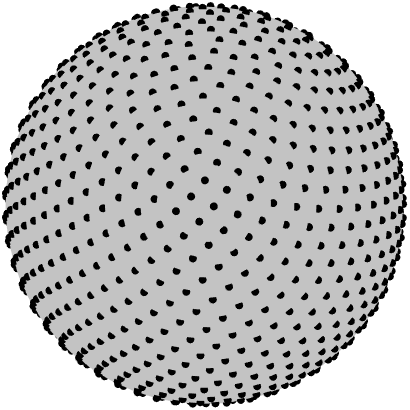
\includegraphics[width=3cm]{5-Figures/Chapter4/fibonacci_sphere/fibonacci_sphere_normal.png}}\hfil   
\subfloat[Top]{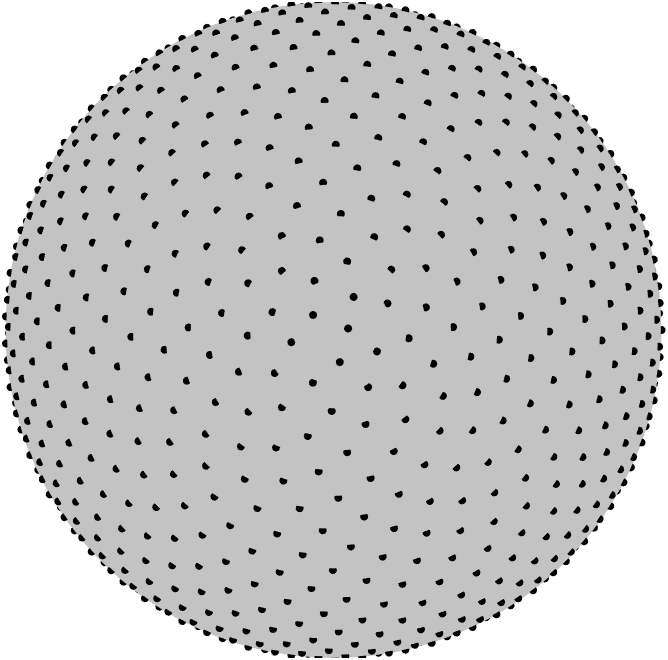
\includegraphics[width=3cm]{5-Figures/Chapter4/fibonacci_sphere/fibonacci_sphere_top.png}}\hfil
\subfloat[Side]{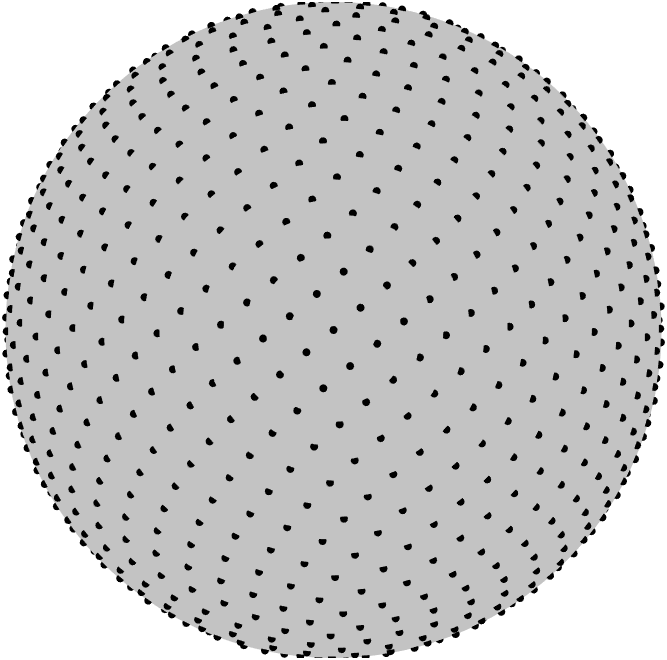
\includegraphics[width=3cm]{5-Figures/Chapter4/fibonacci_sphere/fibonacci_sphere_side.png}}
\caption{Fibonacci Lattice demonstration (1001 points)}
\label{fig.3:fibonacci_lattice_demonstration}
\end{figure}


\subsection{Poisson Disk sampling} \label{sec.3:Poisson sampling disk}

Poisson disk sampling is a stochastic sampling technique that enforces a minimum distance between samples, producing distributions that are both random and well-spaced. Formally, a Poisson disk distribution is defined such that no two samples are closer than a user-defined distance \gls{min_dist}. This property avoids clustering while preserving randomness, resulting in so-called \emph{blue noise} characteristics, which are highly desirable for a very isotropic distribution of agents.

Poisson disk samples are generated using the \textit{fast algorithm} proposed by Bridson\cite{poisson_sampling_disk}. The method improves efficiency by restricting candidate samples to a neighborhood around existing points. A background grid is used to accelerate distance queries, with the cell size chosen as $\gls{min_dist} / \sqrt{n}$ in an $n$-dimensional domain, ensuring that each cell contains at most one sample.

The algorithm starts by placing an initial random sample in the domain and adding it to an active list. While this list is not empty, a sample is selected and up to \gls{P_k} candidate points are generated uniformly in the spherical annulus between radii \( r \) and \( 2r \). If a candidate is at least distance \gls{min_dist} from all existing samples, it is accepted and added to the active list. If no valid candidate is found after \gls{P_k} attempts, the sample is removed from the active list.

Because each iteration either adds or removes a sample and the number of candidate attempts is bounded by a constant, the overall computational complexity of the algorithm is \( O(N) \), being \( N \) the total number of samples. A key advantage of this approach is that it generalizes naturally to arbitrary dimensions, making it well suited for multi-dimensional sampling problems.

It may seem counterintuitive to classify a stochastic sampling technique alongside direct computation methods. However, despite its internal iterative procedure, Poisson disk sampling produces a final, fixed distribution once the algorithm completes. This contrasts with truly iterative methods, where point positions are continuously updated over time to gradually approach an evenly spaced configuration. Since Poisson disk sampling does not involve such progressive adjustment after generation, it is considered, in this work, a direct computation method.

For a desired fixed number of agents \gls{n_D}, a challenge arises because standard Poisson disk sampling does not guarantee an exact number of generated points. To address this limitation, a gradient-based iterative solver might be cable of adjusting minimum separation distance necessary to guarantee a desired number of agents. This refinement might enable the placement of exactly \gls{n_D} agents with approximately uniform spacing. Owing to its low computational cost, such an approach could be practical for real-time or large-scale deployments. However, it should be noted that this remains a conceptual approach and has neither been proven feasible nor experimentally validated during the development of this thesis.

In Figure~\ref{fig.3:poisson_disk_sphere}, the results of this method are visible. This method produces highly isotropic, blue-noise distributions and generalizes naturally to arbitrary manifolds, in this case since the manifold is the two-sphere the usual problem of connection of the "borders" creates clustering on the poles, also take note that the standard Poisson disk sampling does not guarantee an exact number of points, requiring additional refinement if a fixed team size is prescribed. This method also seems viable due to its non uniform distribution being the only main fault as mentioned before the number of agent can not directly be passed to the equation.

\begin{figure}[htbp]
\centering
\subfloat[Normal]{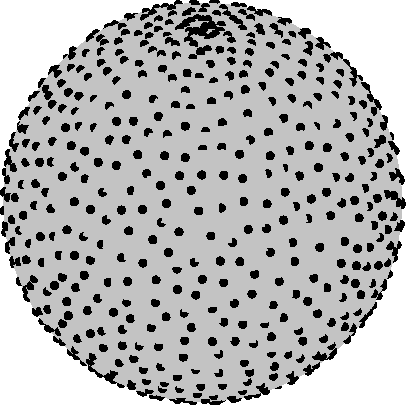
\includegraphics[width=3cm]{5-Figures/Chapter3/poisson_disk/poisson_disk_normal.pdf}}\hfil
\subfloat[Top]{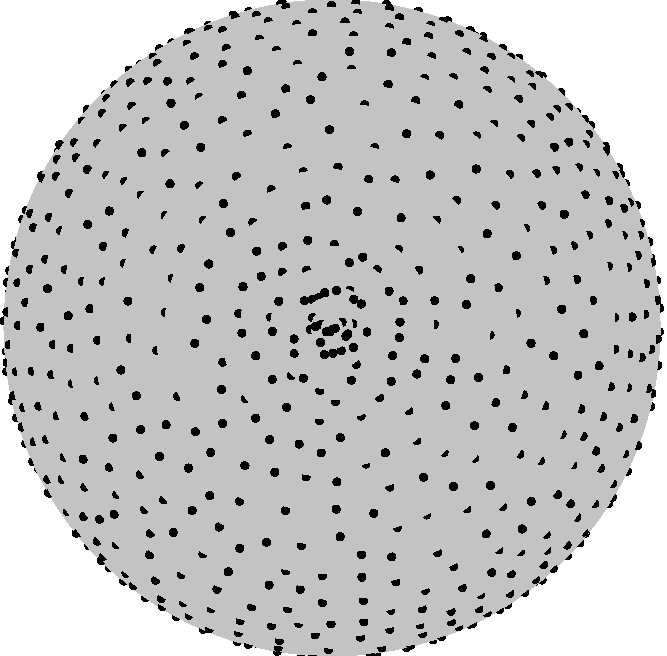
\includegraphics[width=3cm]{5-Figures/Chapter3/poisson_disk/poisson_disk_top.pdf}}\hfil
\subfloat[Side]{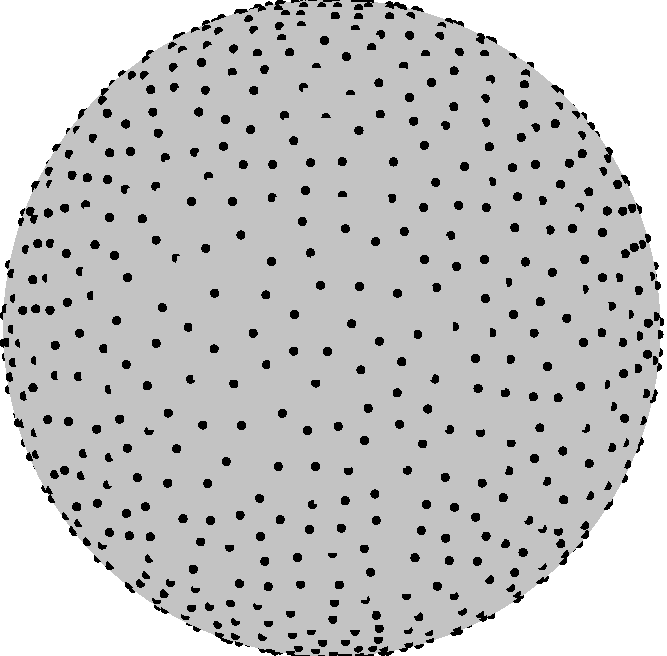
\includegraphics[width=3cm]{5-Figures/Chapter3/poisson_disk/poisson_disk_side.pdf}}
\caption{Poisson disk sampling distribution. (1012 points)}
\label{fig.3:poisson_disk_sphere}
\end{figure}

\section{Iterative computation agent spacing on the two-sphere} \label{sec.3:Iterative computation agent spacing on the two-sphere}

In contrast with the direct computation methods several other iterative computation methods are discussed. This separation between methods comes due to the fact that having iterative methods allows for the use of decentralized implementation of agent spacing that might even not require for every agent to know how many agents exist in the formation as well as not have to agree on the position each agent will take. As in the previous section~\ref{sec.3:Direct computation agent spacing on the two-sphere}, the primary objective is to achieve the most uniform spacing possible between agents. Two different methods are presented, the Thomson minimum energy sphere and Lloyd's algorithm.

\subsection{Thomson minimum energy sphere} \label{sec.3:Thomson minimum energy sphere}

In 1904, J. J. Thomson proposed a model for the atom in which electrons were thought to be evenly distributed within a positively charged sphere. In this model, each electron experiences repulsive forces from the others and is constrained to remain on the surface of the sphere. This concept led to what is now known as the Thomson problem, which seeks the arrangement of $N$ electrons on the surface of a unit sphere that minimizes their total electrostatic potential energy, given that they repel each other according to Coulomb's law. Thomson introduced this problem while developing his atomic model, later called the plum pudding model, reflecting the understanding that negatively charged electrons exist within a neutrally charged atom.\cite{thomson_min_energy_sphere}

The Thomson problem can be formulated mathematically as the minimization of the total Coulomb energy of $N$ point charges constrained to lie on the unit sphere. Let $\mathbf{x}_i \in \mathbb{R}^3$ denote the Cartesian coordinates of the $i$-th point on the sphere, such that $\|\mathbf{x}_i\|_2 = 1$ for all $i = 1, \dots, N$. The total electrostatic potential energy is given by

\begin{equation}
E(\mathbf{X}) = \sum_{i=1}^{N} \sum_{j=i+1}^{N} \frac{1}{\|\mathbf{x}_i - \mathbf{x}_j\|_2},
\end{equation}

where $\mathbf{X} = [\mathbf{x}_1, \mathbf{x}_2, \dots, \mathbf{x}_N] \in \mathbb{R}^{N \times 3}$ is the matrix of all point coordinates, and $\|\mathbf{x}_i - \mathbf{x}_j\|_2$ is the Euclidean distance between points $i$ and $j$. The goal of the Thomson problem is to find

\begin{equation}
\mathbf{X}^* = \arg \min_{\mathbf{X} \in (\mathbb{S}^2)^N} E(\mathbf{X}),
\end{equation}

The only found benefit of using this method, for the desired formation purposes, is that due to there not being any imposed  restrictions, the number of agents on the two-sphere can be any \gls{n_D}, being the downside that this method is extremely slow as will be later demonstrate is Chapter~\ref{cha:Background}. The results of this method can be visible in Figure~\ref{fig.3:thomson_demonstration}.

\begin{figure}[htbp]
    \centering
    \subfloat[Normal]{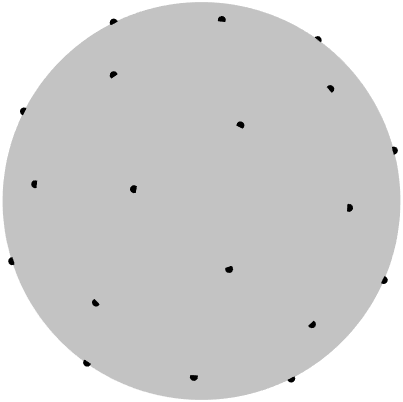
\includegraphics[width=3cm]{5-Figures/Chapter4/thomson_sphere/thomson_normal.png}}\hfil   
    \subfloat[Top]{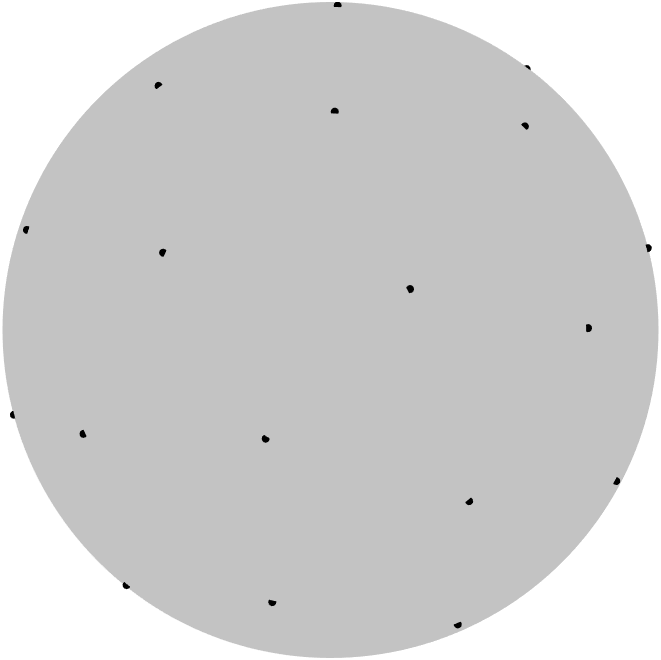
\includegraphics[width=3cm]{5-Figures/Chapter4/thomson_sphere/thomson_top.png}}\hfil
    \subfloat[Side]{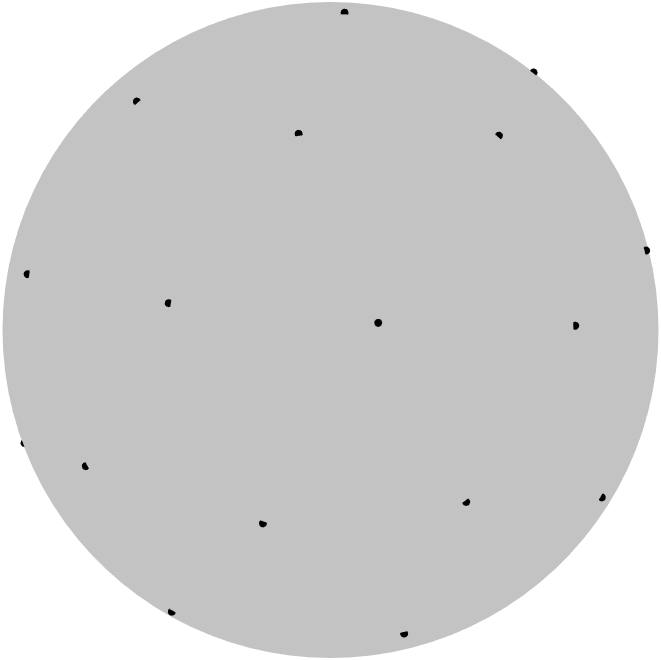
\includegraphics[width=3cm]{5-Figures/Chapter4/thomson_sphere/thomson_side.png}}
    \caption{Thomson demonstration (31 points)}
    \label{fig.3:thomson_demonstration}
\end{figure}

\subsection{Lloyd's algorithm} \label{sec.3:Lloyd's algorithm}

Lloyd's algorithm is an iterative optimization method commonly used to compute \gls{CVT} \cite{duCentroidalVoronoiTessellations1999}, which yield highly uniform point distributions over a domain. The method alternates between partitioning the space into Voronoi regions and relocating each sample point (also called a site) to the centroid of its corresponding region. Both steps can be implemented in multiple ways, some of which are discussed in Section~\ref{subsec.3:Voronoi diagrams}. When applied to the two-sphere, this process produces configurations in which points tend to distribute evenly across the surface, making it well suited for agent spacing problems, the examples of this distribution are shown per method implemented.

\subsection{Voronoi diagrams} \label{subsec.3:Voronoi diagrams}
A Voronoi diagram partitions a metric space into regions based on proximity to a given set of sites. The i-th Voronoi \gls{ith_voronoi_region} region consists of all points that are closer to site \gls{ith_voronoi_centroid} than to any other site.

Formally, let $X$ be a metric space with distance function $d$, which may be Euclidean or geodesic depending on the domain. $K$ be an index set, and \gls{ith_voronoi_centroid}, ${i \in K}$ be a collection of nonempty subsets of $X$ (the sites). The i-th Voronoi region \gls{ith_voronoi_region} associated with the i-th site \gls{ith_voronoi_centroid} is defined as
\begin{equation}
    \gls{ith_voronoi_centroid} = \{ x \in X \mid d(x, \gls{ith_voronoi_centroid}) \leq d(x, c_j) \text{ for all } j \neq i \}.
\end{equation}

Three different methods were implemented to compute both the Voronoi regions and their centroids. For further reading, see \cite{boseSurveyGeodesicPaths2011} for geodesic distance computation and \cite{senechalMathematicalStructuresSpatial1993,aurenhammerVoronoiDiagramsSurvey1991} for Voronoi diagrams.

\paragraph{Voronoi convex hull}

This method calculated the Voronoi region \gls{voronoi_region} from the convex hull, this is a shape that given $N$ points creates the connected edges that will enclose all points in such a way that no point is located outside of the shape. In this case the internal  $\text{MATLAB}^\text{\textregistered}$ \cite{MATLAB:R2024a} function \cite{MATLAB_convhull} is used. With this triangulation of agent position is it possible to calculate the normal to each triangle face plane, which on the unit sphere does correspond to the spherical circumcenter \cite{renkaAlgorithm772STRIPACK1997}. and use them as the voronoi vertices, with the vertices defined it becomes easy to calculate the area of the surface of the Voronoi region \gls{voronoi_region}, since the region is located in the two-sphere the vertices and said triangles of the convex hull are passed to the sphere surface and the area is calculated directly in the manifold using L'Huilier formula. In Figure~\ref{fig.3:Convex_hull_demonstration} it is possible to visualize the created convex hull and Delaunay triangulation for a random formation of 30 points on the two-sphere surface.

\begin{figure}[htbp]
    \centering
    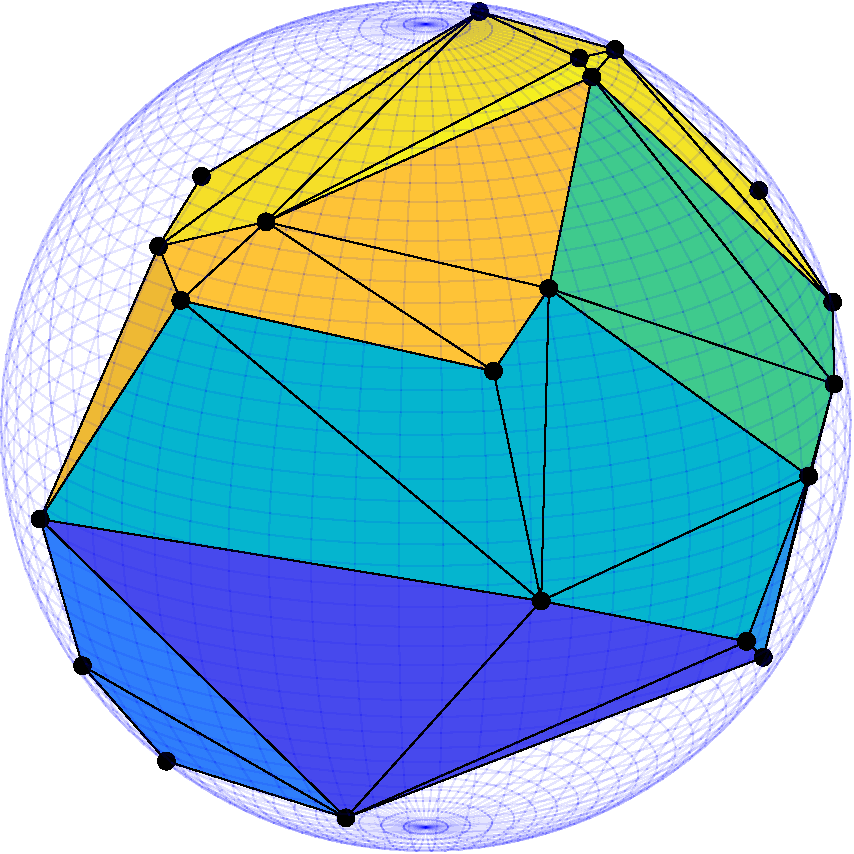
\includegraphics[width=0.8\textwidth]{5-Figures/Chapter3/Lloyd_convex_hull/convex_hull_demonstration.pdf}
    \caption{Convex hull for 30 points}
    \label{fig.3:Convex_hull_demonstration}
\end{figure}

The centroid of the region \gls{voronoi_centroid} is approximated as the weighted average of the sum of the vertices of each triangle, formed by the current centroid and its convex hull vertices, normalized with the area of the given triangle. Formally given by

\begin{equation}
    \gls{voronoi_centroid} \approx 
    \sum_{j=2}^{M-1} 
    A(\mathbf{v}_0, \mathbf{v}_j, \mathbf{v}_{j+1}) \,
    \dfrac{\mathbf{v}_0 + \mathbf{v}_j + \mathbf{v}_{j+1}}
    {\left\| \mathbf{v}_0 + \mathbf{v}_j + \mathbf{v}_{j+1} \right\|}
\end{equation}

being $A$ the area of the triangular surface given by the vertices $v0$, the center vertex, and M the number of vertices composing the edges of the voronoi area of the site $v0$. The new center \gls{voronoi_centroid} becomes the new site and subsequent $v0$ for the next iteration. This algorithm has a computational complexity per iteration of O($kn$) \cite{giffonQuicKmeansAcceleratingInference2021}, being k the number of edges a given point has and n the number of points, being the tital number of iterations necessary for the sites to stabilize dependent on the mesh shape, its resolution and number of agents. 

This method suffers that it required at least 4 agents, this is a hard constraint from the convex hull function and for a small number of agents or some particular formations the algorithm fails and all points collapse to a single position as can be seen in the example given by Figure~\ref{fig.3:Convex_hull_problems} 

\begin{figure}[htbp]
    \centering
    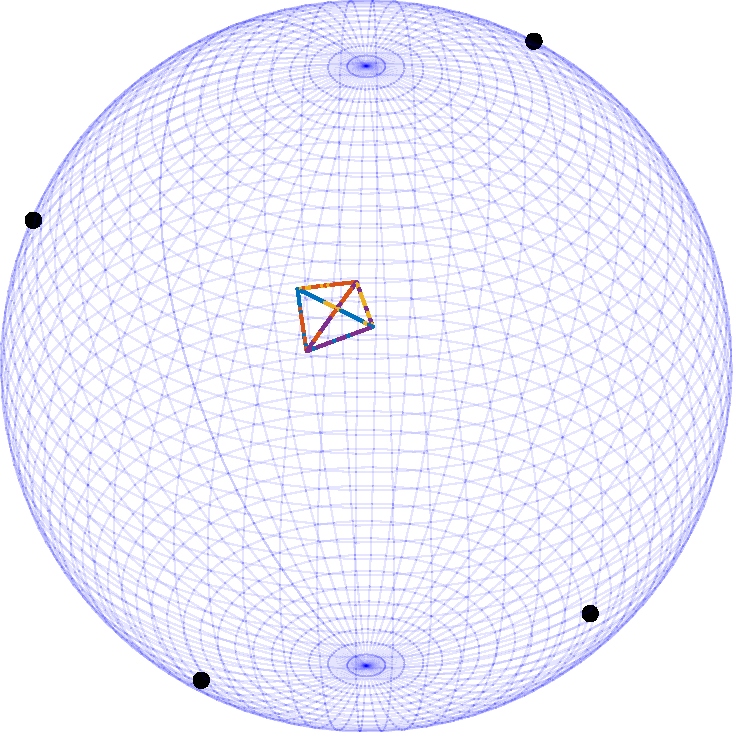
\includegraphics[width=0.8\textwidth]{5-Figures/Chapter3/Lloyd_convex_hull/convex_hull_problems.pdf}
    \caption{Problematic convex hull formation}
    \label{fig.3:Convex_hull_problems}
\end{figure}

What is happening here is that as per design the convex hull creates 4 vertices that separate the Voronoi regions but since the manifold is a closed form two-sphere and the defined implementation always uses the smallest geodesic curve for the area and centroid calculation the geodesic and respective areas are wrongly defined, since they are being defined as the smaller geodesic curve on the sphere and should be defined as the geodesic curve that does almost a full rotation along the sphere, for example it can be seen that the purple line at the bottom of the rectangle shape if extended to connected the two vertices of the geodesic curve via the other side of the sphere, would separate the left top and bottom points. Since the geodesics being considered are the smaller ones, the points will update to inside this rectangular shape in the following iteration, worsening the problem, until all points are situated on the same position.

The results of this methods can be seen in Figure~\ref{fig.3:llyod_convex_hull_algorithm_distribution} showing not only the final position of the points after 300 iteration but also the voronoi lines separating each area. 

\begin{figure}[htbp]
    \centering
    \subfloat[Normal]{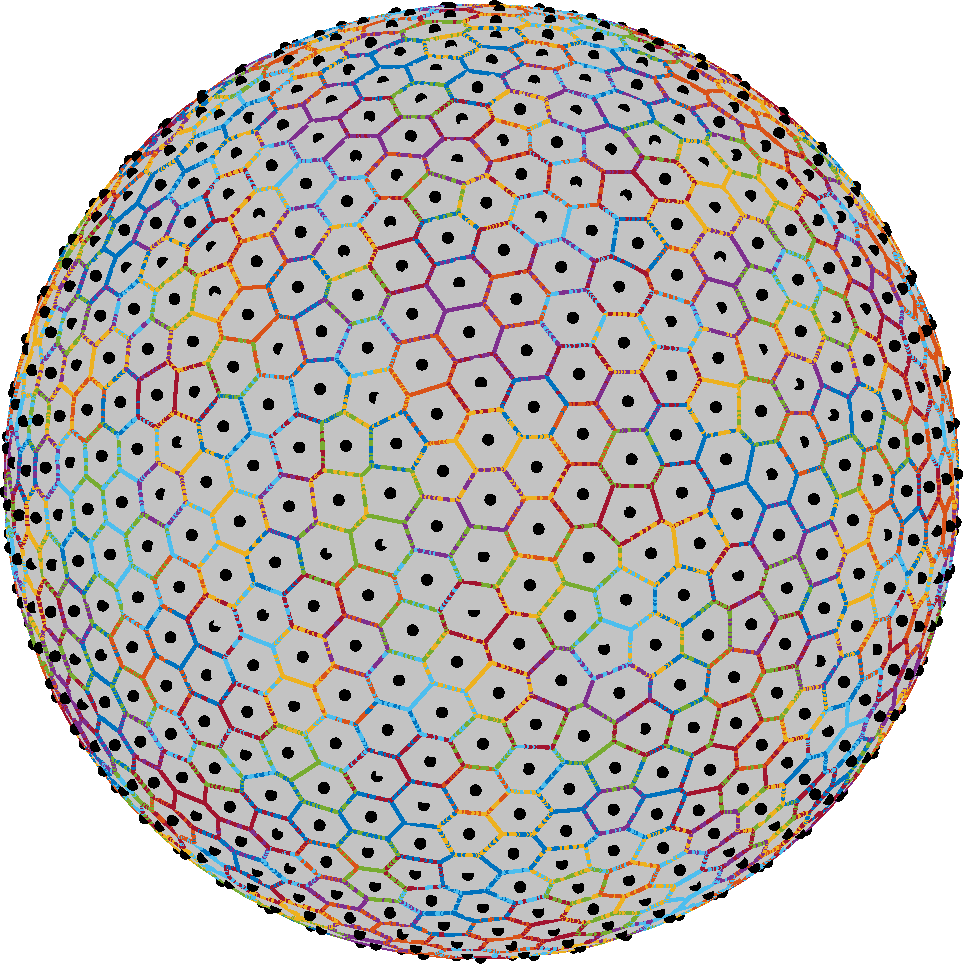
\includegraphics[width=3cm]{5-Figures/Chapter3/Lloyd_convex_hull/Lloyd_normal.pdf}}\hfil
    \subfloat[Top]{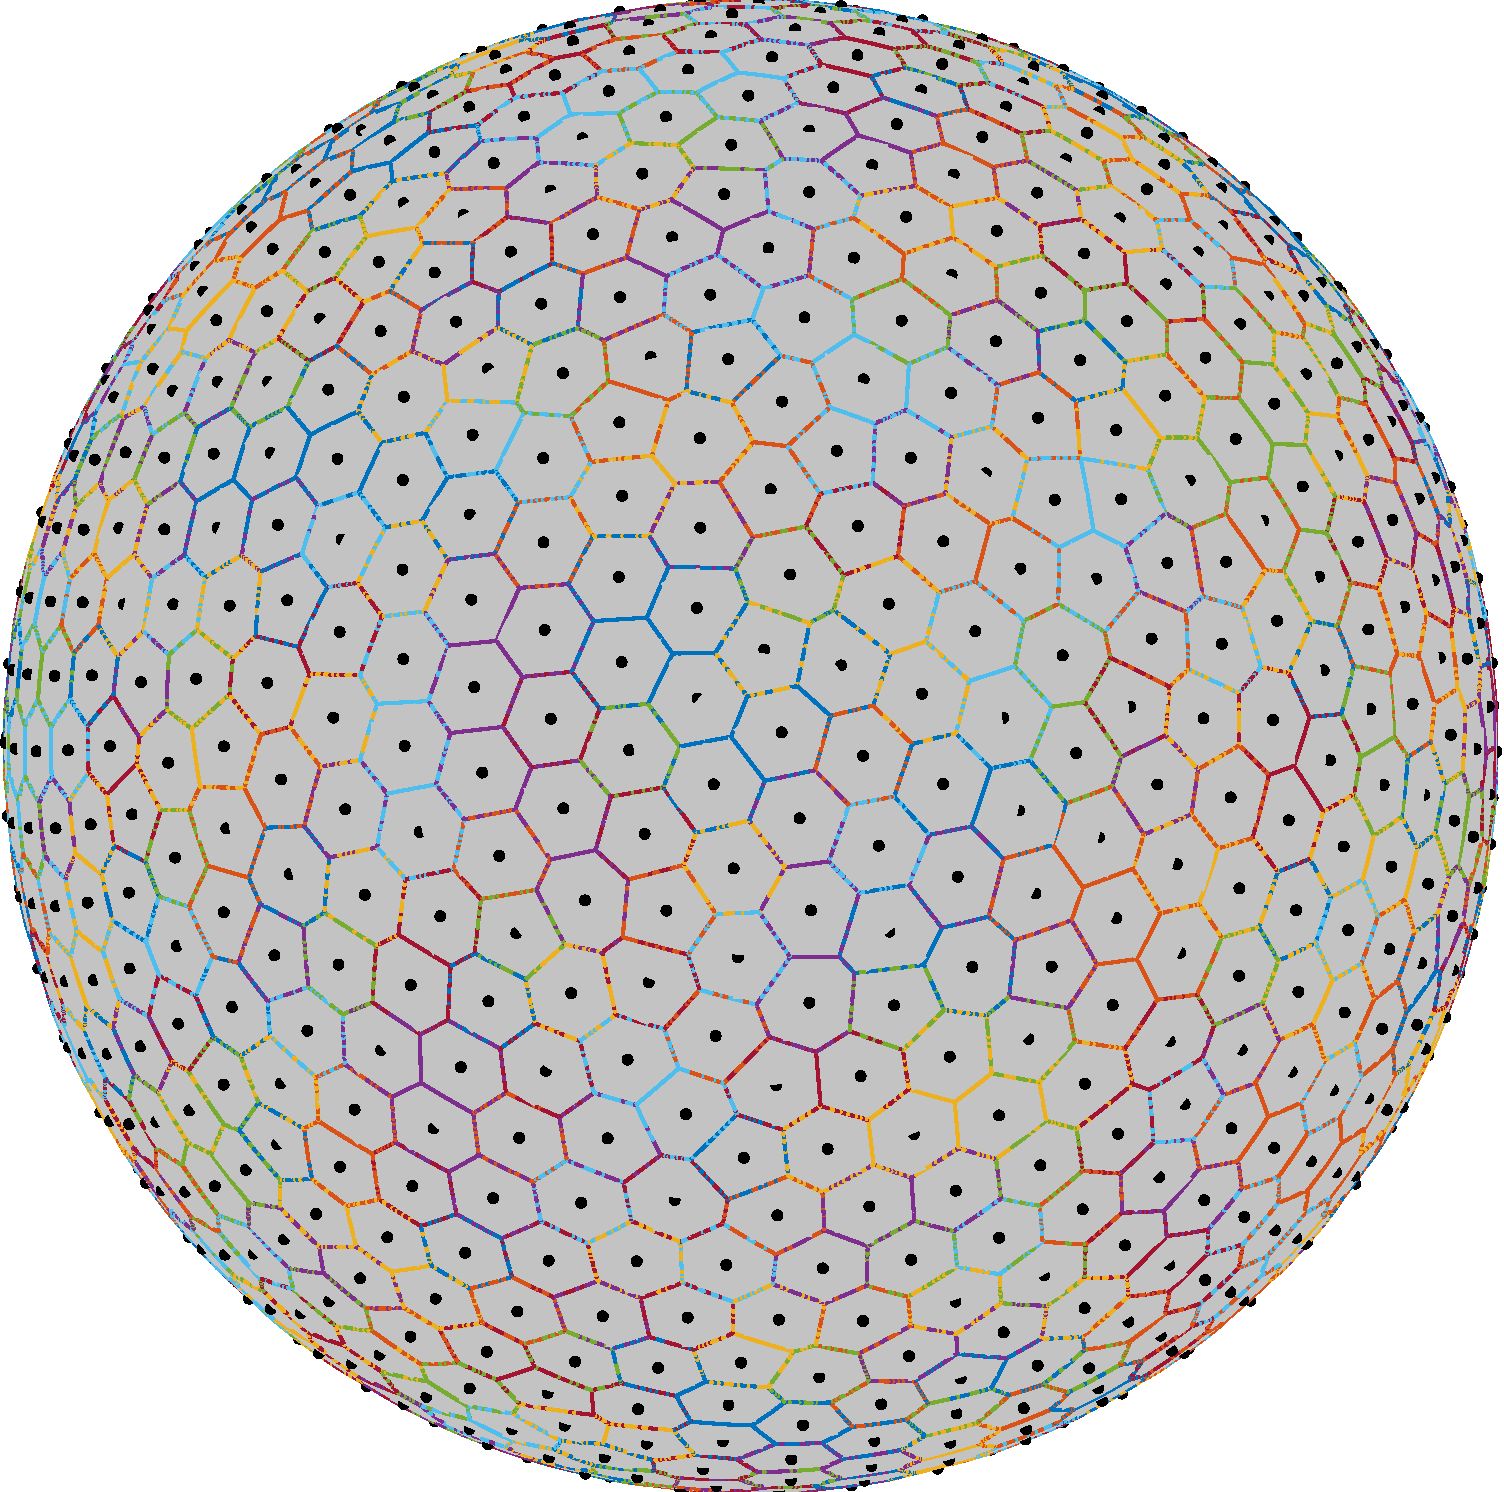
\includegraphics[width=3cm]{5-Figures/Chapter3/Lloyd_convex_hull/Lloyd_top.pdf}}\hfil
    \subfloat[Side]{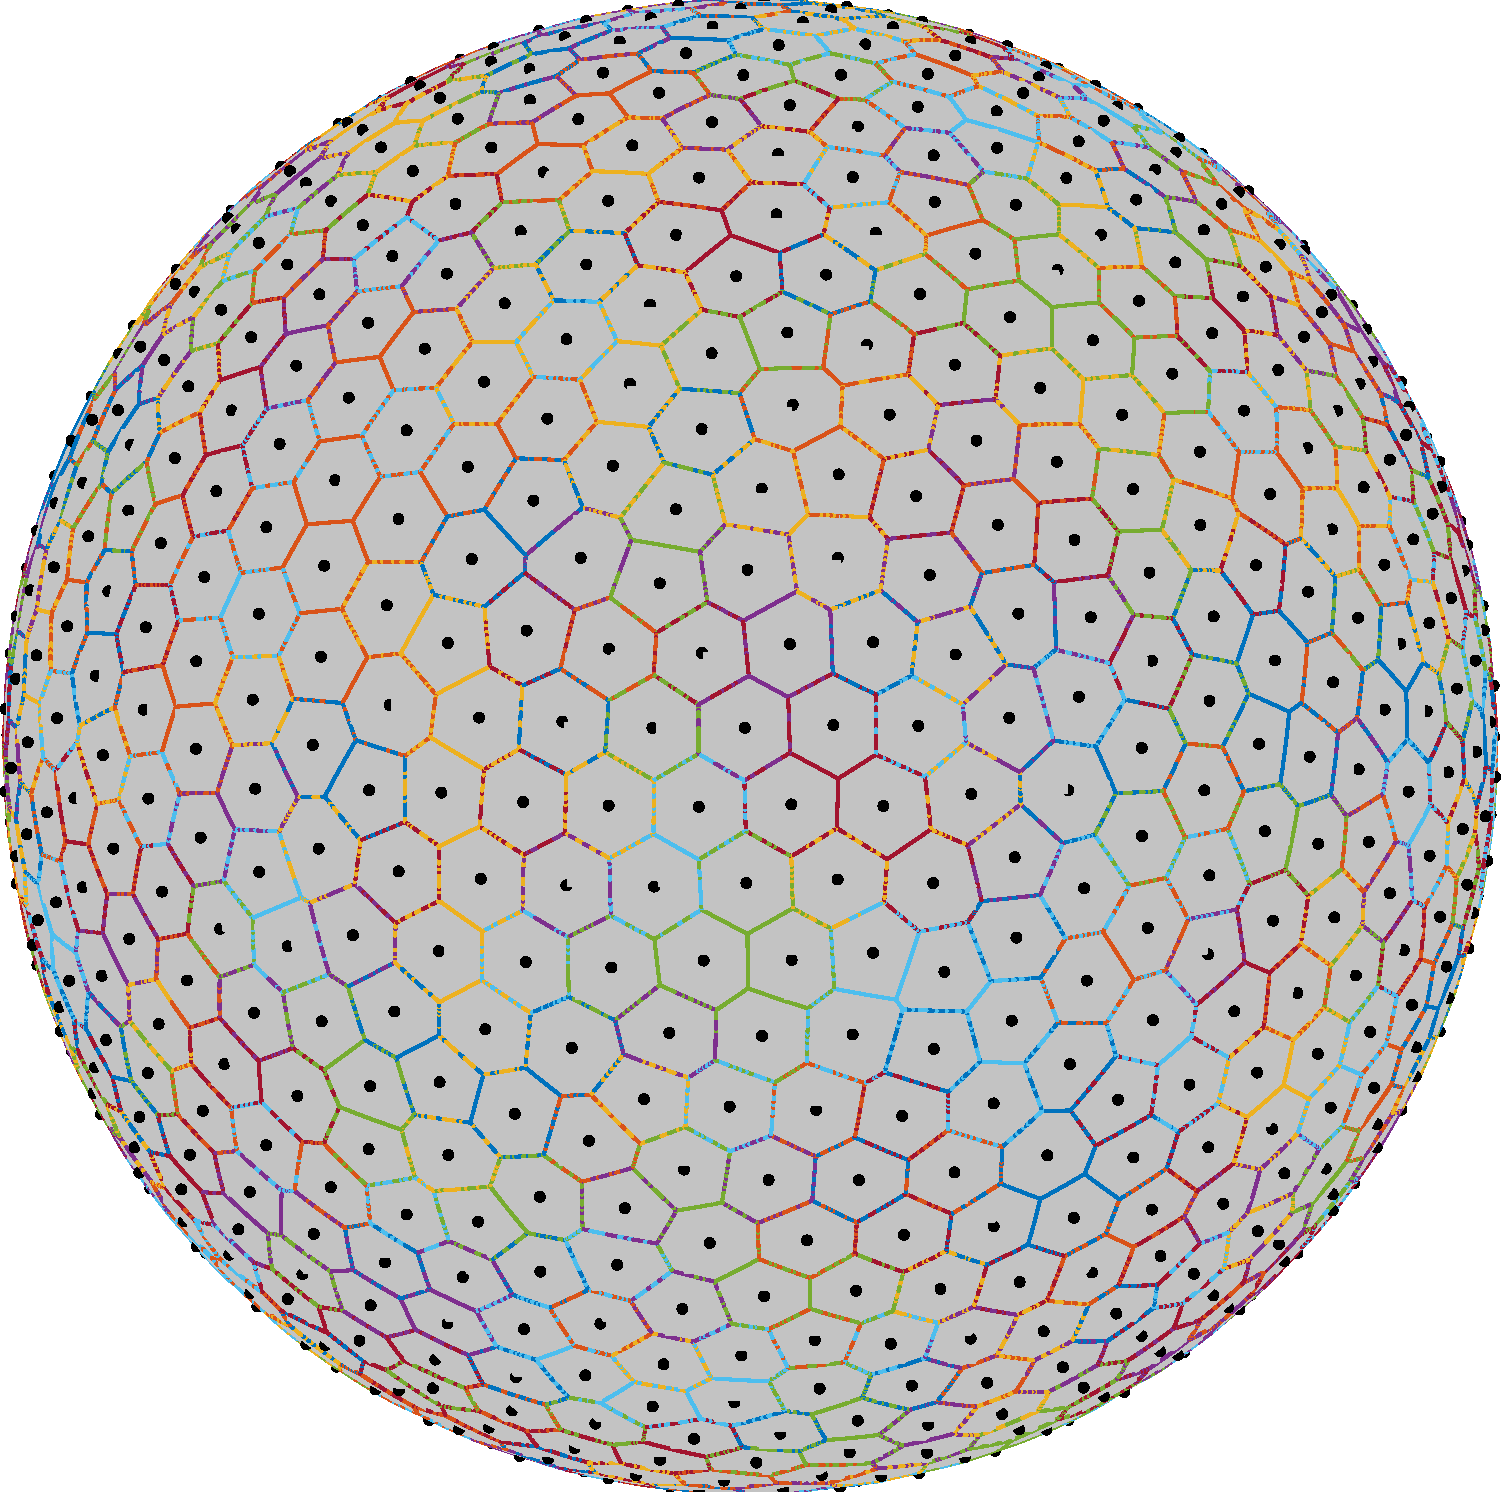
\includegraphics[width=3cm]{5-Figures/Chapter3/Lloyd_convex_hull/Lloyd_side.pdf}}
    \caption{Lloyd's algorithm (convex hull) distribution. (1001 points)}
    \label{fig.3:llyod_convex_hull_algorithm_distribution}
\end{figure}

\paragraph{Voronoi half plane}

The second implementation of Lloyd's algorithm is referred to as the \emph{half-plane method}. In contrast with the convex hull approach, this method is robust for any number of agents and does not suffer from the geometric inconsistencies associated with spherical convex hull constructions. However, this robustness comes at the expense of a higher computational cost, with complexity on the order of $\mathcal{O}(n^2)$ \cite{fanHalfPlaneVoronoiDiagram2011}, being n the number of boundary lines.

The main idea of this method is to construct each Voronoi region \gls{voronoi_region} as the intersection of a set of half-spaces defined on the sphere. For a given agent, its Voronoi cell is obtained by iteratively clipping the sphere using bisector planes defined with respect to its neighboring agents.

More specifically, let $\mathbf{p}_i$ denote the position of the $i$-th agent on the unit sphere and $\mathbf{p}_j$ the position of one of its neighbors. The boundary between these two agents is defined by the set of points on the sphere that are equidistant (in the geodesic sense) to both $\mathbf{p}_i$ and $\mathbf{p}_j$. This boundary corresponds to a great-circle arc, which can be constructed by first computing the geodesic midpoint
\begin{equation}
    \mathbf{m}_{ij} = \frac{\sin((1-\frac{1}{2})\theta)\mathbf{p}_i + \sin(\frac{1}{2}\theta)\mathbf{p}_j}{\sin(\theta)}, \quad \theta = \arccos(\mathbf{p}_i \cdot \mathbf{p}_j),
\end{equation}
and the normal vector to the plane containing both agents
\begin{equation}
    \mathbf{n}_{ij} = \frac{\mathbf{p}_i \times \mathbf{p}_j}{\|\mathbf{p}_i \times \mathbf{p}_j\|}.
\end{equation}

A tangent direction to the bisector at $\mathbf{m}_{ij}$ is then given by
\begin{equation}
    \mathbf{t}_{ij} = \frac{\mathbf{n}_{ij} \times \mathbf{m}_{ij}}{\|\mathbf{n}_{ij} \times \mathbf{m}_{ij}\|}.
\end{equation}

This construction defines a plane passing through $\mathbf{m}_{ij}$ with normal $\mathbf{t}_{ij}$, which splits the sphere into two half-spaces. The Voronoi region associated with agent $i$ is obtained as the intersection of the universe $\Omega$ with all half-spaces defined by the bisecting planes between agent $i$ and all other sites.
\begin{equation}
    V_i
    =
    \Omega
    \cap
    \bigcap_{j \in \mathcal{N}_i}
    \left\{
    \mathbf{x}\in\mathbb{R}^3
    \;\middle|\;
    (\mathbf{x}-\mathbf{m}_{ij})\cdot\mathbf{t}_{ij} < 0
    \right\}.
    \label{eq.3:half_plane_voronoi_calculation}
\end{equation}
where $\mathcal{N}_i$ denotes neighboring sites.

In practice, the region is approximated by discretizing the sphere into a finite set of points and applying all half-plane constraints to determine which points belong to the Voronoi cell. This results in a binary mask over the sphere surface representing the region.

The centroid of the Voronoi region \gls{ith_voronoi_centroid} is then computed numerically by triangulating the valid surface elements of the discretized sphere. Each quadrilateral patch is divided into two triangles, and the centroid is approximated as the area-weighted average of the centroids of these triangles.
\begin{equation}
    \gls{ith_voronoi_centroid} \approx \sum_{i} A_i c_{{\text{triangle}}_i}
\end{equation}

where $A_i$ and $c_{{\text{triangle}}_i}$ denote the area and centroid of the $i$-th triangle parcel making up the Voronoi region. The resulting centroid is then projected back onto the unit sphere.

This method guarantees that the Voronoi regions are correctly defined with respect to geodesic distances on the sphere, avoiding the ambiguity between shorter and longer geodesics that arises in the convex hull approach. Consequently, it provides stable and consistent behavior for Lloyd's algorithm across all configurations, as illustrated in Figure~\ref{fig.3:llyod_half_plane_algorithm_distribution}.

Despite its robustness, the main limitation of this approach is its computational cost. Since each Voronoi region is constructed by evaluating all pairwise half-plane constraints and performing a discretized surface integration, the overall complexity scales quadratically with the number of agents, making it less suitable for large-scale systems, in Figure~\ref{fig.3:llyod_half_plane_algorithm_distribution} it is possible to see the point spacing obtained by this method for 30 points.

\begin{figure}[htbp]
    \centering
    \subfloat[Normal]{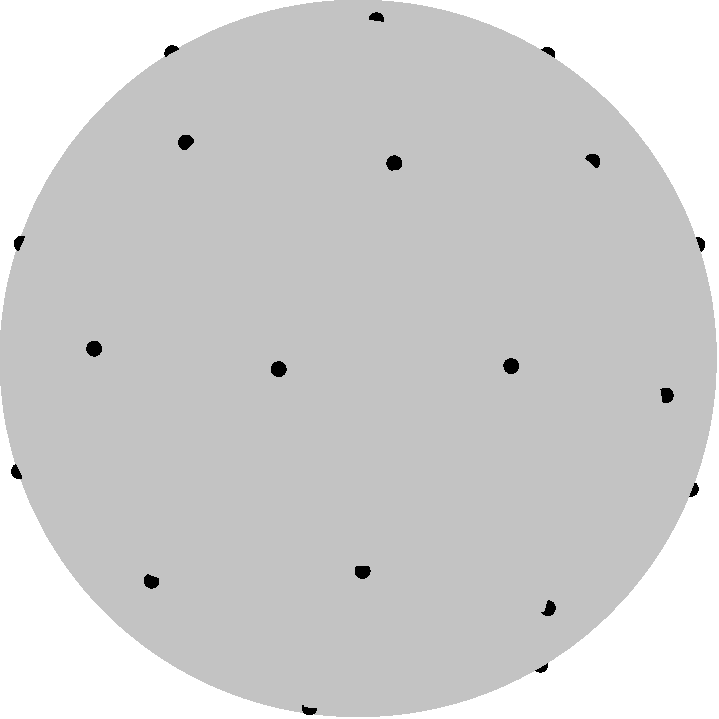
\includegraphics[width=3cm]{5-Figures/Chapter3/Lloyd_half_plane/Lloyd_half_plane_normal.pdf}}\hfil
    \subfloat[Top]{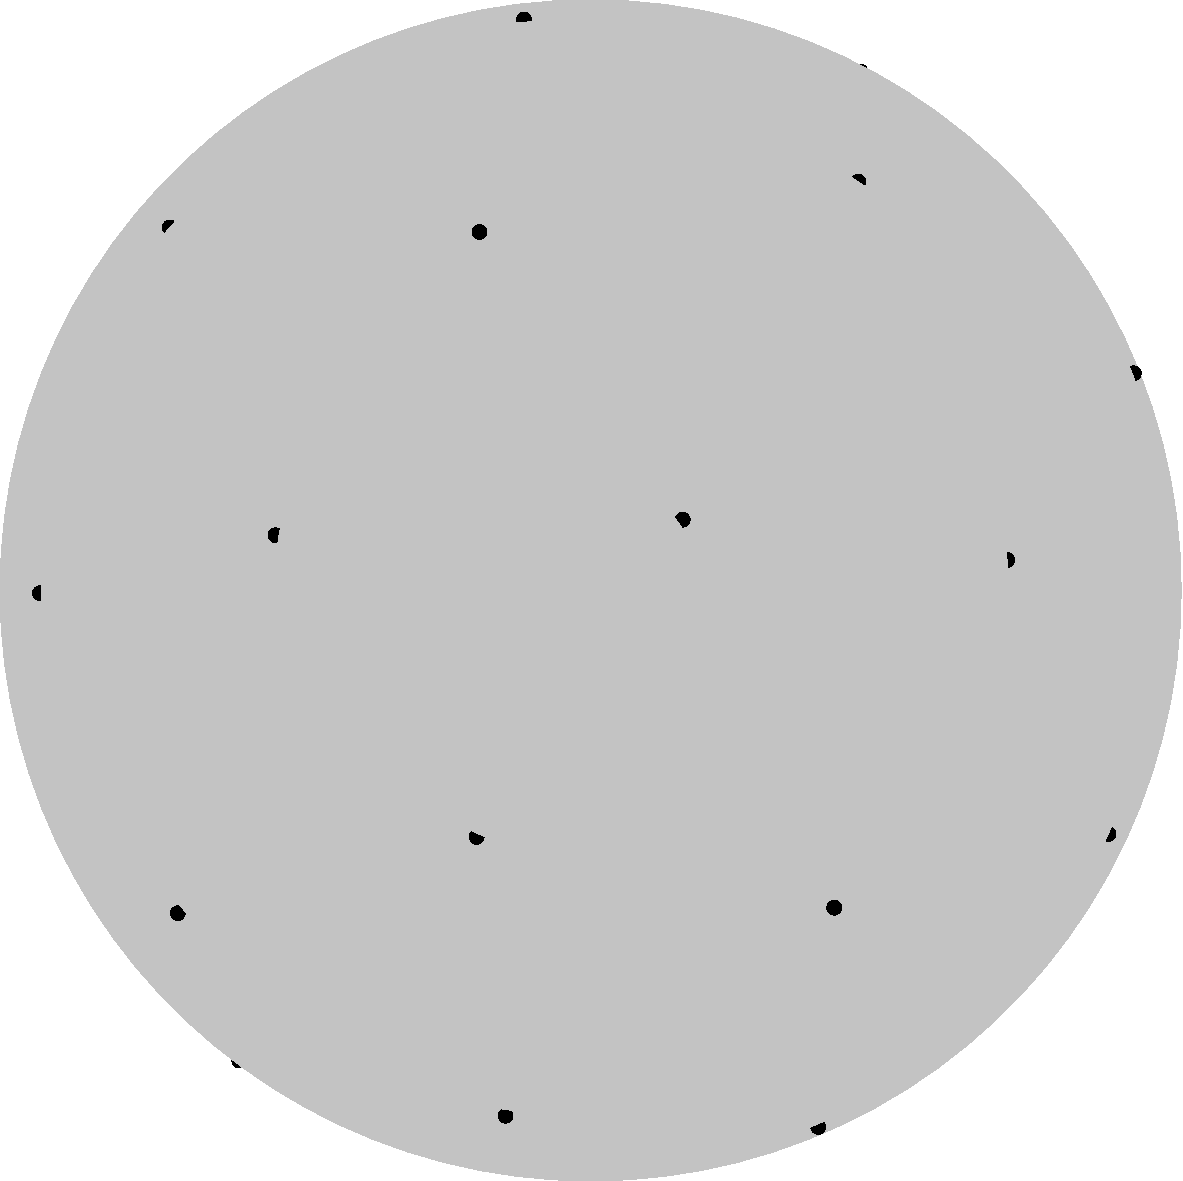
\includegraphics[width=3cm]{5-Figures/Chapter3/Lloyd_half_plane/Lloyd_half_plane_top.pdf}}\hfil
    \subfloat[Side]{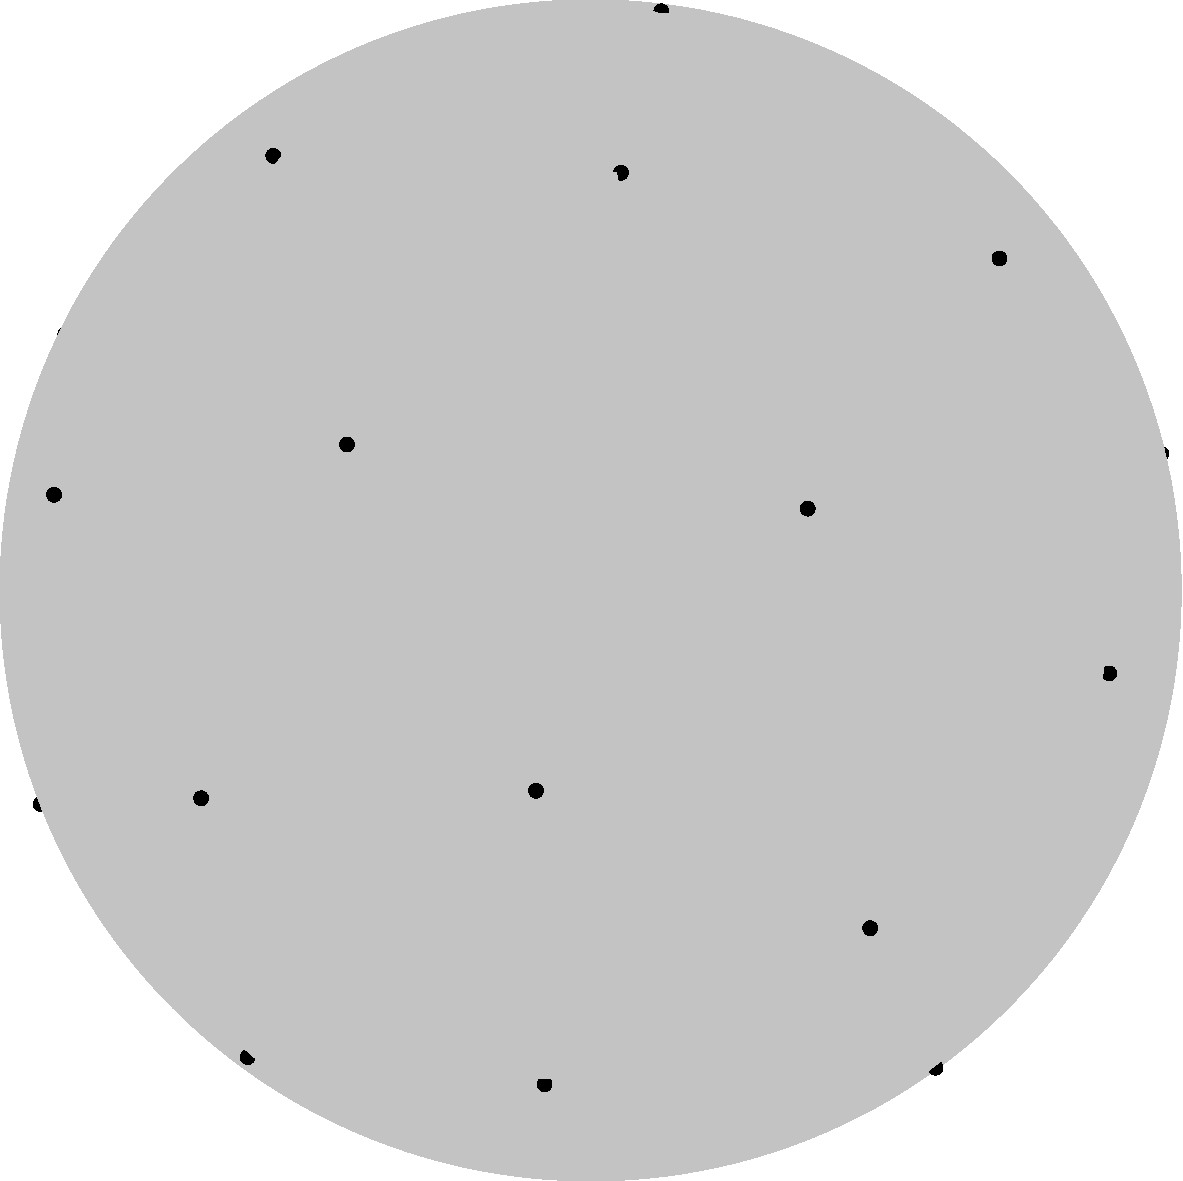
\includegraphics[width=3cm]{5-Figures/Chapter3/Lloyd_half_plane/Lloyd_half_plane_side.pdf}}
    \caption{Lloyd's algorithm (half plane) distribution. (30 points)}
    \label{fig.3:llyod_half_plane_algorithm_distribution}
\end{figure}

\paragraph{Voronoi Dijkstra}
Voronoi separation using the Dijkstra method is a graph-based approach for constructing discrete Voronoi regions on generalized, well-defined meshes. In this framework, the mesh is interpreted as a weighted graph whose vertices correspond to mesh nodes and whose edges encode adjacency, with weights typically derived from geometric properties such as edge lengths or anisotropic metrics.

Given a set of seed points (sites), the algorithm simultaneously propagates fronts from each site across the mesh using Dijkstra's shortest-path procedure. Each vertex is assigned to the site from which it has the minimal geodesic distance, resulting in a partition of the mesh into Voronoi cells.

Voronoi edges are implicitly defined along mesh edges that connect vertices assigned to different sites. In other words, if two adjacent vertices have different nearest sites, the edge between them lies on the boundary between Voronoi regions. Some implementations refine this by detecting where distance fronts from different sites meet or by interpolating along edges to obtain a more precise boundary location. A more complex and complete algorithm than the one implemented in this thesis can be found in \cite{mengEfficientAlgorithmApproximate2023}.

This approach is particularly suitable for irregular or non-Euclidean domains, as it does not rely on explicit geometric constructions but instead leverages the intrinsic connectivity of the mesh. For generalized meshes that are well-defined—i.e., manifolds with consistent connectivity and non-degenerate elements—the method ensures robustness and convergence to a discrete approximation of the continuous Voronoi diagram.

\begin{figure}[htbp]
    \centering
    \subfloat[Normal]{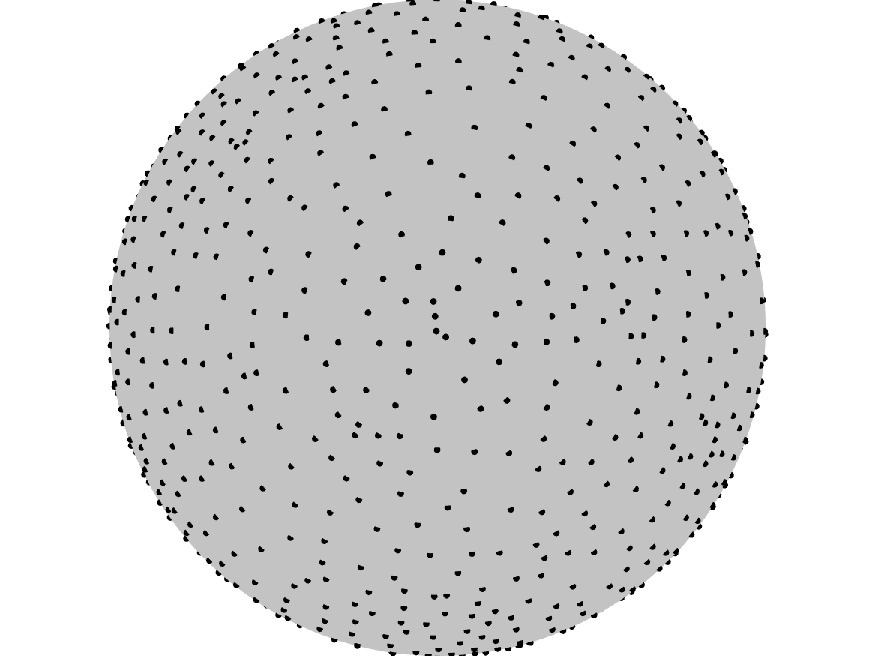
\includegraphics[width=3cm]{5-Figures/Chapter3/Lloyd_disktra/Voronoi_dijkstra_normal.pdf}}\hfil
    \subfloat[Top]{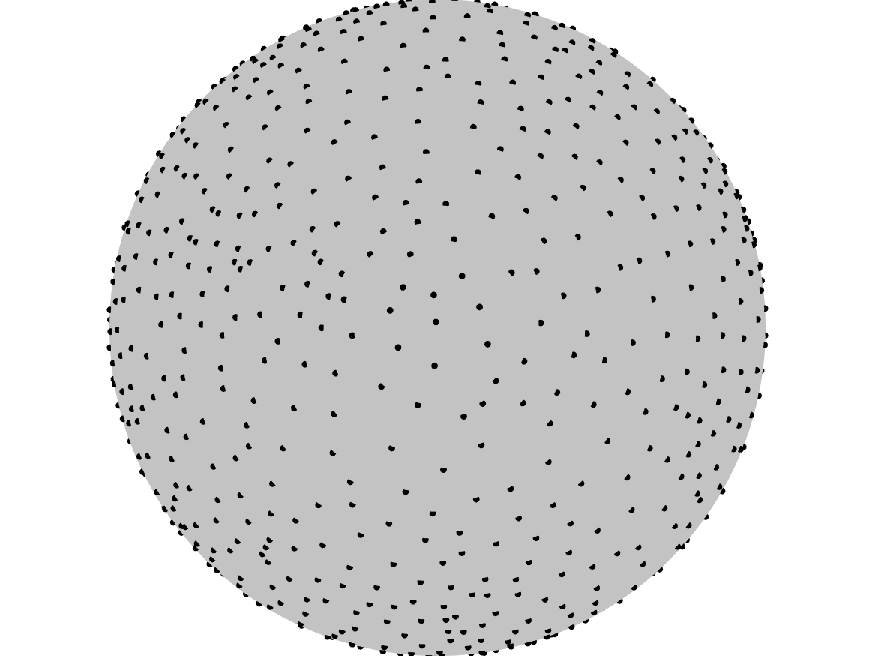
\includegraphics[width=3cm]{5-Figures/Chapter3/Lloyd_disktra/Voronoi_dijkstra_top.pdf}}\hfil
    \subfloat[Side]{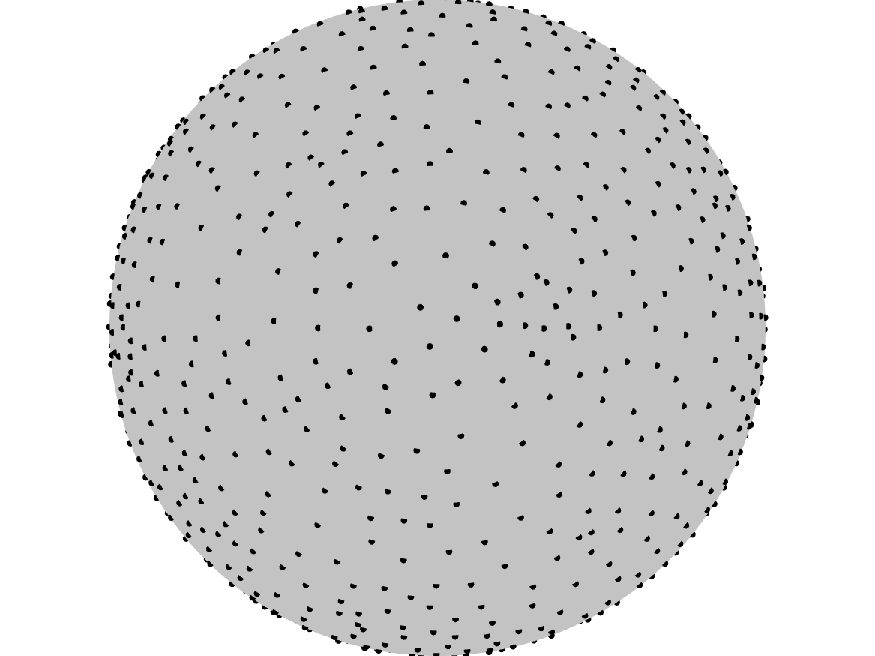
\includegraphics[width=3cm]{5-Figures/Chapter3/Lloyd_disktra/Voronoi_dijkstra_side.pdf}}
    \caption{Lloyd's algorithm (dijkstra) distribution. (1001 points)}
    \label{fig.3:llyod_dijkstra_algorithm_distribution}
\end{figure}

\section{Vehicle model and nonlinear control}
\label{sec.3:Vehicle model and noninear control}

The \gls{RUAV}, obtained from \cite{AlexandraGonalvesRodrigues2023}, is modeled as a rigid body with six
degrees of freedom evolving in \gls{3D} space. Two reference frames are
considered: the body frame \gls{drone_body_matrix}$\{e_1, e_2, e_3\}$ attached
to the vehicle's center of mass and the inertial frame \gls{drone_inertial_matrix}$\{E_1, E_2, E_3\}$, being also defined \gls{drone_mass} as the mass of the drone, and \gls{gravity} the gravity acceleration.

The position and velocity of the RUAV in the inertial frame are given by \gls{chaser_pos} and \gls{chaser_vel} while the orientation and angular velocity are given by \gls{chaser_ori} and \gls{chaser_ang_vel}.

The \gls{UAV} model can be written as:
\begin{equation}
\begin{aligned}
\dot{\gls{chaser_pos}} &= \gls{chaser_vel} \\
\dot{\gls{chaser_ori}} &= E(\gls{chaser_ori})^{-1}\,\omega_{B_D} \\
\dot{\gls{chaser_vel}} &= \gls{drone_mass}^{-1} R_{IB}(\gls{chaser_ori})\,(\gls{p_force} + \gls{p_drag_force}) - \gls{gravity}\, R_{IB}(\gls{chaser_ori})^{T} e_3 \\
\dot{\omega}_{B_D} &= \gls{drone_inertial_matrix}^{-1}\!\left(-\omega_{B_D} \times (I \omega_{B_D}) + \gls{p_torque} + \gls{p_drag_torque} \right)
\end{aligned}
\end{equation}

The rotation matrix $R_{IB}(\Phi)$ and Jacobian $E(\Phi)$ are shown in Equation~\eqref{eq.3:rotation_matrix} and Equation~\eqref{eq.3:jacobian_matrix} respectively, where for simplicity $c=\cos(\cdot)$, $s=\sin(\cdot)$, $t=\tan(\cdot)$.

\begin{equation}
R_{IB}(\Phi) =
\begin{bmatrix}
c_\theta c_\psi &
c_\theta s_\psi &
- s_\theta \\
s_\phi s_\theta c_\psi - c_\phi s_\psi &
s_\phi s_\theta s_\psi + c_\phi c_\psi &
s_\phi c_\theta \\
c_\phi s_\theta c_\psi + s_\phi s_\psi &
c_\phi s_\theta s_\psi - s_\phi c_\psi &
c_\phi c_\theta
\end{bmatrix}
\label{eq.3:rotation_matrix}
\end{equation}

\begin{equation}
E(\Phi)^{-1} =
\begin{bmatrix}
1 & s_\phi t_\theta & c_\phi t_\theta \\
0 & c_\phi & -s_\phi \\
0 & \dfrac{s_\phi}{c_\theta} & \dfrac{c_\phi}{c_\theta}
\end{bmatrix}
\label{eq.3:jacobian_matrix}
\end{equation}

The aerodynamic drag force \gls{p_drag_force} and torque \gls{p_drag_torque} produced by aerodynamic drag are, respectively,$ \gls{p_drag_force} = - \mathrm{diag}(a_T, a_T, a_T) R_{IB}(\Psi)^{T} v_{air}$ with $v_{air} = v_a - v_w$, where $v_w$ is the wind velocity vector in the inertial frame, and $\gls{p_drag_torque} = - \mathrm{diag}(a_R, a_R, a_R)\boldsymbol{\omega}_a$ where $a_t$ and $a_r$ are the linear and rotational air friction, respectively. For the external force \gls{p_force} and torque \gls{p_torque} we have
\begin{equation}
\mathbf{f}_e =
\begin{bmatrix}
0 & 0 & f_{ez}
\end{bmatrix}^{T},
\qquad
\boldsymbol{\tau}_e =
\begin{bmatrix}
\tau_{ex} & \tau_{ey} & \tau_{ez}
\end{bmatrix}^{T}.
\end{equation}

A compact notation for the continuous equation of the model can be defined as 

\begin{equation}
\dot{\mathbf{x}}(t) = \mathbf{f} \bigl( \mathbf{x}(t), \mathbf{u}(t) \bigr).
\tag{3.4}
\end{equation} 
This full nonlinear model is used throughout the rest of this thesis for simulation and control design, providing a realistic representation of the \gls{RUAV} dynamics, and is controlled via a nonlinear internal controller derived from the work of Daniel Mellinger and Vijay Kumar \cite{Mellinger2011}, for simplicity referred from this point on as the "Mellinger Controller". The controller receives as inputs the desired position \gls{p_desired}, velocity \gls{v_desired}, and attitude \gls{a_desired} \cite{AlexandraGonalvesRodrigues2023, Crazyflie_mellinger}, and computes the required thrust commands for each motor of a quadrotor. Figure~\ref{fig.3:mellinger_controller_architecture} illustrates the architecture of the Mellinger Controller, where the Position Controller gives the desired force $F^\star$ and the Attitude Controller the actuation torque \gls{p_drag_torque}.

\begin{figure}[htbp]
  \centering
  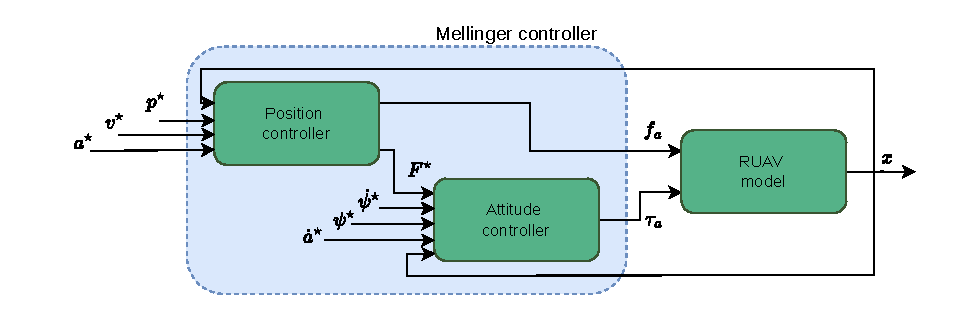
\includegraphics[width=\textwidth]{5-Figures/Chapter3/Mellinger Controller.pdf}
  \caption{Mellinger Controller}
  \label{fig.3:mellinger_controller_architecture}
\end{figure}

\section{Lyapunov Stability and Lyapunov-Based Control} \label{sec.3:Lyapunov Stability and Lyapunov-Based Control}

Lyapunov theory provides a rigorous framework for analyzing the stability of nonlinear dynamical systems and for designing stabilizing control laws without the need to explicitly solve the system equations. In this work, Lyapunov-based methods are employed to analyze and ensure the stability of a reduced-attitude control system evolving on manifolds. A brief introduction to Lyapunov control is presented, with a particular focus on the Lyapunov controller proposed in \cite{lyapunov_outer_loop_control} and its formal definition. This section summarizes the Lyapunov-based reduced-attitude control framework introduced in \cite{lyapunov_outer_loop_control}, which serves as the mathematical foundation for the higher-level control strategy developed in the subsequent sections of this thesis.

\subsection{System Description}

Consider a nonlinear dynamical system of the form

\begin{equation}
    \dot{\mathbf{x}} = \mathbf{f}(\mathbf{x}, \mathbf{u}),
\end{equation}

where $\mathbf{x} \in \mathbb{R}^n$ denotes the system state and $\mathbf{u} \in \mathbb{R}^m$ is the control input.  
An equilibrium point $\mathbf{x}_e$ satisfies $\mathbf{f}(\mathbf{x}_e, \mathbf{u}_e) = \mathbf{0}$ and can be shifted to the origin via an appropriate change of variables.

\subsection{Lyapunov Stability and Control}

Let $V : \mathbb{R}^n \rightarrow \mathbb{R}$ be a continuously differentiable, positive-definite function with $V(\mathbf{0}) = 0$.  
If its time derivative along system trajectories satisfies
\begin{equation}
    \dot{V}(\mathbf{x}) \le 0,
\end{equation}
then the equilibrium is Lyapunov stable. If $\dot{V}(\mathbf{x}) < 0$ for all $\mathbf{x} \neq \mathbf{0}$, asymptotic stability is ensured.

In Lyapunov-based control, the control law $\mathbf{u}(\mathbf{x})$ is designed such that the closed-loop dynamics yield a non-increasing Lyapunov function, guaranteeing stability by construction. This approach is particularly suitable for nonlinear systems evolving on manifolds, such as rigid-body attitude dynamics.

\subsection{Artificial Potential Fields} \label{sec.3:Artificial Potential Fields}

\gls{APF} are a widely used method for motion planning
and collision avoidance in multi-agent systems. The main idea is to model the
motion of each agent as if it were influenced by an artificial potential field,
where attractive potentials pull the agent toward desired goals and repulsive
potentials push it away from obstacles or other agents.

Let $q_i \in \mathbb{R}^n$ denote the position of agent $i$. The total artificial
potential $U_i(q_i)$ is typically defined as the sum of an attractive potential
$U_i^{\mathrm{att}}$ and a repulsive potential $U_i^{\mathrm{rep}}$,
\begin{equation}
    U_i(q_i) = U_i^{\mathrm{att}}(q_i) + U_i^{\mathrm{rep}}(q_i).
\end{equation}

The control input is then obtained as the negative gradient of the potential,
\begin{equation}
    u_i = - \nabla_{q_i} U_i(q_i),
\end{equation}
which drives the agent toward lower potential energy.

\paragraph{Attractive Potential}

A common choice for the attractive potential toward a desired reference
$q_i^{\mathrm{ref}}$ is a quadratic function,
\begin{equation}
    U_i^{\mathrm{att}}(q_i) =
    \frac{1}{2} k_{\mathrm{att}} \| q_i - q_i^{\mathrm{ref}} \|^2,
\end{equation}
where $k_{\mathrm{att}} > 0$ is a gain parameter. The corresponding
attractive force is
\begin{equation}
    u_i^{\mathrm{att}} =
    - \nabla_{q_i} U_i^{\mathrm{att}} =
    - k_{\mathrm{att}} (q_i - q_i^{\mathrm{ref}}).
\end{equation}

\paragraph{Repulsive Potential}

To avoid collisions, a repulsive potential is introduced between agent $i$
and neighboring agents $j$. Let $d_{ij} = \| q_i - q_j \|$ denote the distance
between agents. A typical repulsive potential is defined as
\begin{equation}
    U_i^{\mathrm{rep}} =
    \sum_{j \neq i}
    \begin{cases}
        \frac{1}{2} k_{\mathrm{rep}}
        \left( \frac{1}{d_{ij}} - \frac{1}{d_0} \right)^2,
        & d_{ij} < d_0, \\[6pt]
        0, & d_{ij} \ge d_0,
    \end{cases}
\end{equation}
where $k_{\mathrm{rep}} > 0$ is a gain and $d_0$ is the influence distance
beyond which no repulsion is applied.

The corresponding repulsive force is
\begin{equation}
    u_i^{\mathrm{rep}} =
    - \nabla_{q_i} U_i^{\mathrm{rep}} =
    \sum_{j \neq i}
    \begin{cases}
        k_{\mathrm{rep}}
        \left( \frac{1}{d_{ij}} - \frac{1}{d_0} \right)
        \frac{1}{d_{ij}^2}
        \frac{q_i - q_j}{d_{ij}},
        & d_{ij} < d_0, \\[6pt]
        0, & d_{ij} \ge d_0.
    \end{cases}
\end{equation}

The resulting control input applied to agent $i$ is the combination of
attractive and repulsive components,
\begin{equation}
    u_i = u_i^{\mathrm{att}} + u_i^{\mathrm{rep}}.
\end{equation}

\gls{APF} methods are attractive due to their simplicity, decentralization, and
low computational cost. However, they suffer from well-known limitations,
including the presence of local minima, oscillatory behavior near obstacles,
and the lack of formal guarantees on collision avoidance. Despite these
limitations, APFs remain a practical and widely adopted solution  \cite{litimeinSurveyTechniquesCircular2021} \cite{colomboQuantumRiemannianCubics2026} for real-time
multi-agent navigation and are often combined with other techniques to improve
robustness and safety.

\section{Network topologies} \label{sec.3:Network topologies}

Several classes of network topologies and associated consensus algorithms have been studied in the literature \cite{olfati-saberConsensusCooperationNetworked2007} to determine a suitable structure for decentralized multi-agent coordination. Among these, spatially induced networks \cite{cortesRobustRendezvousMobile2006} are particularly well-suited for systems in which agents are embedded in a physical environment and interactions are constrained by proximity.

In this work, the communication topology is constructed using Delaunay triangulation, which naturally defines neighbor relationships based on the spatial distribution of agents. This approach ensures that the resulting graph is sparse, planar, and connected under mild conditions, while avoiding overly long communication links.

To account for agent motion and improve information flow, the network is allowed to vary over time by recomputing the triangulation. This rewiring process yields a dynamic topology that preserves connectivity while promoting efficient information mixing across the network. As a result, the time-varying structure enhances convergence performance in practical decentralized implementations.

\section{Consensus-Based Coordination} \label{sec.3:Consensus-Based Coordination}

Consensus-based coordination is a fundamental approach in multi-agent systems, where a group of agents cooperatively achieves a common objective through local interactions.
Typical applications include formation control, distributed estimation, flocking, and cooperative robotics.
The key idea is that global coordination emerges from simple local interaction rules defined by the communication network.

\subsection{Graph-Theoretic Representation}

The interaction topology of a multi-agent system is commonly modeled using graph theory.
Let the communication network be represented by a graph
\begin{equation}
    \mathcal{G} = (\mathcal{V}, \mathcal{E}),
\end{equation}
where $\mathcal{V} = \{1,2,\dots,N\}$ is the set of nodes (agents) and $\mathcal{E} \subseteq \mathcal{V} \times \mathcal{V}$ is the set of edges representing information exchange.

If information flow between agents is bidirectional, the graph is undirected; otherwise, directed.
The connectivity properties of $\mathcal{G}$ play a crucial role in determining whether consensus can be achieved.

The \textit{adjacency matrix} $\mathbf{A} \in \mathbb{R}^{N \times N}$ characterizes the local interactions among agents.
Its elements are defined as
\begin{equation}
    a_{ij} =
    \begin{cases}
        w_{ij} > 0, & \text{if agent $j$ sends information to agent $i$}, \\
        0, & \text{otherwise},
    \end{cases}
\end{equation}
where $w_{ij}$ denotes the weight of the communication link.
For undirected graphs, $\mathbf{A}$ is symmetric.

The adjacency matrix determines which agents influence each other and with what relative strength.
However, it does not explicitly capture the notion of disagreement between agents, which is central to consensus dynamics.

The \textit{graph Laplacian matrix} encodes both the adjacency structure and the degree of each node.
It is defined as
\begin{equation}
    \mathbf{L} = \mathbf{D} - \mathbf{A},
\end{equation}
where $\mathbf{D} = \text{diag}(d_1, \dots, d_N)$ is the degree matrix with
\begin{equation}
    d_i = \sum_{j=1}^{N} a_{ij}.
\end{equation}

The Laplacian matrix plays a central role in consensus analysis.
It has the following important properties:
\begin{itemize}
    \item $\mathbf{L}\mathbf{1} = \mathbf{0}$, where $\mathbf{1}$ is the vector of all ones.
    \item All eigenvalues of $\mathbf{L}$ are non-negative.
    \item The multiplicity of the zero eigenvalue equals the number of connected components of the graph.
\end{itemize}

For undirected and connected graphs, $\mathbf{L}$ has a single zero eigenvalue, which is a necessary and sufficient condition for consensus.

\subsection{Consensus Algorithms}

Consider a group of $N$ agents, each with scalar state $x_i \in \mathbb{R}$.
A standard continuous-time consensus protocol is given by
\begin{equation}
    \dot{x}_i = \sum_{j=1}^{N} a_{ij} (x_j - x_i),
\end{equation}
which can be written in compact form as
\begin{equation}
    \dot{\mathbf{x}} = -\mathbf{L}\mathbf{x}.
\end{equation}

This dynamics drives the agents toward a common value by reducing the disagreement between neighboring states.
If the communication graph is connected, all states converge to a consensus value
\begin{equation}
    \lim_{t \to \infty} x_i(t) = x^\ast, \quad \forall i.
\end{equation}

For undirected graphs, the consensus value corresponds to the average of the initial states.
The convergence rate is influenced by the second smallest eigenvalue of the Laplacian, known as the \textit{algebraic connectivity}. An example of a consensus algorithm can be seen in \cite{Jin2018}, where a consensus algorithm is used in order for given a circular topology all agents obtain the same center around which to form a circle.

\subsection{Exponential Moving Average} \label{sec.3:Exponential Moving Average}

The \gls{EMA} is a widely used method in finances \cite{raudysMovingAveragesFinancial2013} that incorporates both past estimates and new observations. It computes a weighted sum between the previous estimate and the new measurement, as shown in Equation~\eqref{eq:exponential moving avereaga}.

\begin{equation}
    EMA_{\text{estimate}} = (1 - \alpha_{\text{EMA}})\, EMA_{\text{estimate}} + \alpha_{\text{EMA}} \cdot \text{measurement}
    \label{eq:exponential moving avereaga}
\end{equation}

where $\alpha_{\text{EMA}} \in (0,1)$ is the smoothing factor that determines the relative importance of the new measurement compared to the previous estimate.

\subsection{Extensions and Remarks}

Consensus algorithms can be extended to higher-order agent dynamics, time-varying topologies, directed graphs, and delayed communication.
Despite these complexities, the Laplacian matrix remains the fundamental tool for analyzing stability and convergence.
As a result, consensus-based coordination provides a scalable and fully distributed framework for multi-agent control systems. \cite{4118472, 1431045, 1205192}